
%%%%%%%%%%%%%%%%%% PREAMBULE %%%%%%%%%%%%%%%%%%

\documentclass[aspectratio=169,utf8]{beamer}
%\documentclass[aspectratio=169,handout]{beamer}

\usetheme{Boadilla}
%\usecolortheme{seahorse}
\usecolortheme[RGB={245,66,24}]{structure}
\useoutertheme{infolines}

% packages
\usepackage{amsfonts,amsmath,amssymb,amsthm}
\usepackage[utf8]{inputenc}
\usepackage[T1]{fontenc}
\usepackage{lmodern}

\usepackage[francais]{babel}
\usepackage{fancybox}
\usepackage{graphicx}

\usepackage{float}
\usepackage{xfrac}

%\usepackage[usenames, x11names]{xcolor}
\usepackage{tikz}
\usepackage{pgfplots}
\usepackage{datetime}



%-----  Package unités -----
\usepackage{siunitx}
\sisetup{locale = FR,detect-all,per-mode = symbol}

%\usepackage{mathptmx}
%\usepackage{fouriernc}
%\usepackage{newcent}
%\usepackage[mathcal,mathbf]{euler}

%\usepackage{palatino}
%\usepackage{newcent}
% \usepackage[mathcal,mathbf]{euler}



% \usepackage{hyperref}
% \hypersetup{colorlinks=true, linkcolor=blue, urlcolor=blue,
% pdftitle={Exo7 - Exercices de mathématiques}, pdfauthor={Exo7}}


%section
% \usepackage{sectsty}
% \allsectionsfont{\bf}
%\sectionfont{\color{Tomato3}\upshape\selectfont}
%\subsectionfont{\color{Tomato4}\upshape\selectfont}

%----- Ensembles : entiers, reels, complexes -----
\newcommand{\Nn}{\mathbb{N}} \newcommand{\N}{\mathbb{N}}
\newcommand{\Zz}{\mathbb{Z}} \newcommand{\Z}{\mathbb{Z}}
\newcommand{\Qq}{\mathbb{Q}} \newcommand{\Q}{\mathbb{Q}}
\newcommand{\Rr}{\mathbb{R}} \newcommand{\R}{\mathbb{R}}
\newcommand{\Cc}{\mathbb{C}} 
\newcommand{\Kk}{\mathbb{K}} \newcommand{\K}{\mathbb{K}}

%----- Modifications de symboles -----
\renewcommand{\epsilon}{\varepsilon}
\renewcommand{\Re}{\mathop{\text{Re}}\nolimits}
\renewcommand{\Im}{\mathop{\text{Im}}\nolimits}
%\newcommand{\llbracket}{\left[\kern-0.15em\left[}
%\newcommand{\rrbracket}{\right]\kern-0.15em\right]}

\renewcommand{\ge}{\geqslant}
\renewcommand{\geq}{\geqslant}
\renewcommand{\le}{\leqslant}
\renewcommand{\leq}{\leqslant}
\renewcommand{\epsilon}{\varepsilon}

%----- Fonctions usuelles -----
\newcommand{\ch}{\mathop{\text{ch}}\nolimits}
\newcommand{\sh}{\mathop{\text{sh}}\nolimits}
\renewcommand{\tanh}{\mathop{\text{th}}\nolimits}
\newcommand{\cotan}{\mathop{\text{cotan}}\nolimits}
\newcommand{\Arcsin}{\mathop{\text{arcsin}}\nolimits}
\newcommand{\Arccos}{\mathop{\text{arccos}}\nolimits}
\newcommand{\Arctan}{\mathop{\text{arctan}}\nolimits}
\newcommand{\Argsh}{\mathop{\text{argsh}}\nolimits}
\newcommand{\Argch}{\mathop{\text{argch}}\nolimits}
\newcommand{\Argth}{\mathop{\text{argth}}\nolimits}
\newcommand{\pgcd}{\mathop{\text{pgcd}}\nolimits} 


%----- Commandes divers ------
\newcommand{\ii}{\mathrm{i}}
\newcommand{\dd}{\text{d}}
\newcommand{\id}{\mathop{\text{id}}\nolimits}
\newcommand{\Ker}{\mathop{\text{Ker}}\nolimits}
\newcommand{\Card}{\mathop{\text{Card}}\nolimits}
\newcommand{\Vect}{\mathop{\text{Vect}}\nolimits}
\newcommand{\Mat}{\mathop{\text{Mat}}\nolimits}
\newcommand{\rg}{\mathop{\text{rg}}\nolimits}
\newcommand{\tr}{\mathop{\text{tr}}\nolimits}


%----- Structure des exercices ------

\newtheoremstyle{styleexo}% name
{2ex}% Space above
{3ex}% Space below
{}% Body font
{}% Indent amount 1
{\bfseries} % Theorem head font
{}% Punctuation after theorem head
{\newline}% Space after theorem head 2
{}% Theorem head spec (can be left empty, meaning ‘normal’)

%\theoremstyle{styleexo}
\newtheorem{exo}{Exercice}
\newtheorem{ind}{Indications}
\newtheorem{cor}{Correction}


\newcommand{\exercice}[1]{} \newcommand{\finexercice}{}
%\newcommand{\exercice}[1]{{\tiny\texttt{#1}}\vspace{-2ex}} % pour afficher le numero absolu, l'auteur...
\newcommand{\enonce}{\begin{exo}} \newcommand{\finenonce}{\end{exo}}
\newcommand{\indication}{\begin{ind}} \newcommand{\finindication}{\end{ind}}
\newcommand{\correction}{\begin{cor}} \newcommand{\fincorrection}{\end{cor}}

\newcommand{\noindication}{\stepcounter{ind}}
\newcommand{\nocorrection}{\stepcounter{cor}}

\newcommand{\fiche}[1]{} \newcommand{\finfiche}{}
\newcommand{\titre}[1]{\centerline{\large \bf #1}}
\newcommand{\addcommand}[1]{}
\newcommand{\video}[1]{}

% Marge
\newcommand{\mymargin}[1]{\marginpar{{\small #1}}}

\def\noqed{\renewcommand{\qedsymbol}{}}


%----- Presentation ------
\setlength{\parindent}{0cm}

%\newcommand{\ExoSept}{\href{http://exo7.emath.fr}{\textbf{\textsf{Exo7}}}}

\definecolor{myred}{rgb}{0.93,0.26,0}
\definecolor{myorange}{rgb}{0.97,0.58,0}
\definecolor{myyellow}{rgb}{1,0.86,0}

\newcommand{\LogoExoSept}[1]{  % input : echelle
{\usefont{U}{cmss}{bx}{n}
\begin{tikzpicture}[scale=0.1*#1,transform shape]
  \fill[color=myorange] (0,0)--(4,0)--(4,-4)--(0,-4)--cycle;
  \fill[color=myred] (0,0)--(0,3)--(-3,3)--(-3,0)--cycle;
  \fill[color=myyellow] (4,0)--(7,4)--(3,7)--(0,3)--cycle;
  \node[scale=5] at (3.5,3.5) {Exo7};
\end{tikzpicture}}
}


\newcommand{\debutmontitre}{
  \author{} \date{} 
  \thispagestyle{empty}
  \hspace*{-10ex}
  \begin{minipage}{\textwidth}
    \titlepage  
  \vspace*{-2.5cm}
  \begin{center}
    \LogoExoSept{2.5}
  \end{center}
  \end{minipage}

  \vspace*{-0cm}
  
  % Astuce pour que le background ne soit pas discrétisé lors de la conversion pdf -> png
\begin{tikzpicture}
        \fill[opacity=0,green!60!black] (0,0)--++(0,0)--++(0,0)--++(0,0)--cycle; 
\end{tikzpicture}

% toc S'affiche trop tot :
% \tableofcontents[hideallsubsections, pausesections]
}

\newcommand{\finmontitre}{
  \end{frame}
  \setcounter{framenumber}{0}
} % ne marche pas pour une raison obscure

%----- Commandes supplementaires ------

% \usepackage[landscape]{geometry}
% \geometry{top=1cm, bottom=3cm, left=2cm, right=10cm, marginparsep=1cm
% }
% \usepackage[a4paper]{geometry}
% \geometry{top=2cm, bottom=2cm, left=2cm, right=2cm, marginparsep=1cm
% }

%\usepackage{standalone}


% New command Arnaud -- november 2011
\setbeamersize{text margin left=24ex}
% si vous modifier cette valeur il faut aussi
% modifier le decalage du titre pour compenser
% (ex : ici =+10ex, titre =-5ex

\theoremstyle{definition}
%\newtheorem{proposition}{Proposition}
%\newtheorem{exemple}{Exemple}
%\newtheorem{theoreme}{Théorème}
%\newtheorem{lemme}{Lemme}
%\newtheorem{corollaire}{Corollaire}
%\newtheorem*{remarque*}{Remarque}
%\newtheorem*{miniexercice}{Mini-exercices}
%\newtheorem{definition}{Définition}

% Commande tikz
\usetikzlibrary{calc}
\usetikzlibrary{patterns,arrows}
\usetikzlibrary{matrix}
\usetikzlibrary{fadings} 

%definition d'un terme
\newcommand{\defi}[1]{{\color{myorange}\textbf{\emph{#1}}}}
\newcommand{\evidence}[1]{{\color{blue}\textbf{\emph{#1}}}}
\newcommand{\assertion}[1]{\emph{\og#1\fg}}  % pour chapitre logique
%\renewcommand{\contentsname}{Sommaire}
\renewcommand{\contentsname}{}
\setcounter{tocdepth}{2}



%------ Figures ------

\def\myscale{1} % par défaut 
\newcommand{\myfigure}[2]{  % entrée : echelle, fichier figure
\def\myscale{#1}
\begin{center}
\footnotesize
{#2}
\end{center}}


%------ Encadrement ------

\usepackage{fancybox}


\newcommand{\mybox}[1]{
\setlength{\fboxsep}{7pt}
\begin{center}
\shadowbox{#1}
\end{center}}

\newcommand{\myboxinline}[1]{
\setlength{\fboxsep}{5pt}
\raisebox{-10pt}{
\shadowbox{#1}
}
}

%--------------- Commande beamer---------------
\newcommand{\beameronly}[1]{#1} % permet de mettre des pause dans beamer pas dans poly


\setbeamertemplate{navigation symbols}{}
\setbeamertemplate{footline}  % tiré du fichier beamerouterinfolines.sty
{
  \leavevmode%
  \hbox{%
  \begin{beamercolorbox}[wd=.333333\paperwidth,ht=2.25ex,dp=1ex,center]{author in head/foot}%
    % \usebeamerfont{author in head/foot}\insertshortauthor%~~(\insertshortinstitute)
    \usebeamerfont{section in head/foot}{\bf\insertshorttitle}
  \end{beamercolorbox}%
  \begin{beamercolorbox}[wd=.333333\paperwidth,ht=2.25ex,dp=1ex,center]{title in head/foot}%
    \usebeamerfont{section in head/foot}{\bf\insertsectionhead}
  \end{beamercolorbox}%
  \begin{beamercolorbox}[wd=.333333\paperwidth,ht=2.25ex,dp=1ex,right]{date in head/foot}%
    % \usebeamerfont{date in head/foot}\insertshortdate{}\hspace*{2em}
    \insertframenumber{} / \inserttotalframenumber\hspace*{2ex} 
  \end{beamercolorbox}}%
  \vskip0pt%
}


\definecolor{mygrey}{rgb}{0.5,0.5,0.5}
\setlength{\parindent}{0cm}
%\DeclareTextFontCommand{\helvetica}{\fontfamily{phv}\selectfont}

% background beamer
\definecolor{couleurhaut}{rgb}{0.85,0.9,1}  % creme
\definecolor{couleurmilieu}{rgb}{1,1,1}  % vert pale
\definecolor{couleurbas}{rgb}{0.85,0.9,1}  % blanc
\setbeamertemplate{background canvas}[vertical shading]%
[top=couleurhaut,middle=couleurmilieu,midpoint=0.4,bottom=couleurbas] 
%[top=fondtitre!05,bottom=fondtitre!60]



\makeatletter
\setbeamertemplate{theorem begin}
{%
  \begin{\inserttheoremblockenv}
  {%
    \inserttheoremheadfont
    \inserttheoremname
    \inserttheoremnumber
    \ifx\inserttheoremaddition\@empty\else\ (\inserttheoremaddition)\fi%
    \inserttheorempunctuation
  }%
}
\setbeamertemplate{theorem end}{\end{\inserttheoremblockenv}}

\newenvironment{theoreme}[1][]{%
   \setbeamercolor{block title}{fg=structure,bg=structure!40}
   \setbeamercolor{block body}{fg=black,bg=structure!10}
   \begin{block}{{\bf Th\'eor\`eme }#1}
}{%
   \end{block}%
}


\newenvironment{proposition}[1][]{%
   \setbeamercolor{block title}{fg=structure,bg=structure!40}
   \setbeamercolor{block body}{fg=black,bg=structure!10}
   \begin{block}{{\bf Proposition }#1}
}{%
   \end{block}%
}

\newenvironment{corollaire}[1][]{%
   \setbeamercolor{block title}{fg=structure,bg=structure!40}
   \setbeamercolor{block body}{fg=black,bg=structure!10}
   \begin{block}{{\bf Corollaire }#1}
}{%
   \end{block}%
}

\newenvironment{mydefinition}[1][]{%
   \setbeamercolor{block title}{fg=structure,bg=structure!40}
   \setbeamercolor{block body}{fg=black,bg=structure!10}
   \begin{block}{{\bf Définition} #1}
}{%
   \end{block}%
}

\newenvironment{lemme}[0]{%
   \setbeamercolor{block title}{fg=structure,bg=structure!40}
   \setbeamercolor{block body}{fg=black,bg=structure!10}
   \begin{block}{\bf Lemme}
}{%
   \end{block}%
}

\newenvironment{remarque}[1][]{%
   \setbeamercolor{block title}{fg=black,bg=structure!20}
   \setbeamercolor{block body}{fg=black,bg=structure!5}
   \begin{block}{Remarque #1}
}{%
   \end{block}%
}


\newenvironment{exemple}[1][]{%
   \setbeamercolor{block title}{fg=black,bg=structure!20}
   \setbeamercolor{block body}{fg=black,bg=structure!5}
   \begin{block}{{\bf Exemple }#1}
}{%
   \end{block}%
}


\newenvironment{miniexercice}[0]{%
   \setbeamercolor{block title}{fg=structure,bg=structure!20}
   \setbeamercolor{block body}{fg=black,bg=structure!5}
   \begin{block}{Mini-exercices}
}{%
   \end{block}%
}


\newenvironment{tp}[0]{%
   \setbeamercolor{block title}{fg=structure,bg=structure!40}
   \setbeamercolor{block body}{fg=black,bg=structure!10}
   \begin{block}{\bf Travaux pratiques}
}{%
   \end{block}%
}
\newenvironment{exercicecours}[1][]{%
   \setbeamercolor{block title}{fg=structure,bg=structure!40}
   \setbeamercolor{block body}{fg=black,bg=structure!10}
   \begin{block}{{\bf Exercice }#1}
}{%
   \end{block}%
}
\newenvironment{algo}[1][]{%
   \setbeamercolor{block title}{fg=structure,bg=structure!40}
   \setbeamercolor{block body}{fg=black,bg=structure!10}
   \begin{block}{{\bf Algorithme}\hfill{\color{gray}\texttt{#1}}}
}{%
   \end{block}%
}


\setbeamertemplate{proof begin}{
   \setbeamercolor{block title}{fg=black,bg=structure!20}
   \setbeamercolor{block body}{fg=black,bg=structure!5}
   \begin{block}{{\footnotesize Démonstration}}
   \footnotesize
   \smallskip}
\setbeamertemplate{proof end}{%
   \end{block}}
\setbeamertemplate{qed symbol}{\openbox}


\makeatother
\usecolortheme[RGB={192,41,0}]{structure}

% Commande spécifique à ce chapitre
\usetikzlibrary{arrows}
\usetikzlibrary{patterns}

\newcommand{\Sage}{\texttt{Sage}}

\usepackage{textcomp}

\usepackage{listings}
\lstset{
  upquote=true,
  columns=flexible,
  keepspaces=true,
  basicstyle=\ttfamily,
  commentstyle=\color{gray},
  language=Python,
  showstringspaces=false,
  aboveskip=0em,  
  belowskip=0em,
  escapeinside=||,
  breaklines=true,
  postbreak=\raisebox{0ex}[0ex][0ex]{\qquad\ensuremath{\color{red}\hookrightarrow\space}},
}

\lstset{
  literate={é}{{\'e}}1
           {è}{{\`e}}1
           {à}{{\`a}}1
}

\newcommand{\codeinline}[1]{\lstinline!#1!}

   
%%%%%%%%%%%%%%%%%%%%%%%%%%%%%%%%%%%%%%%%%%%%%%%%%%%%%%%%%%%%%
%%%%%%%%%%%%%%%%%%%%%%%%%%%%%%%%%%%%%%%%%%%%%%%%%%%%%%%%%%%%%


\begin{document}

\renewcommand*{\theenumii}{\alph{enumii}}

\title{{\bf Calcul formel}}
\subtitle{\'Equations différentielles}

\begin{frame}
  
  \debutmontitre

  \pause

{\footnotesize
\hfill
\setbeamercovered{transparent=50}
\begin{minipage}{0.6\textwidth}
  \begin{itemize}
    \item<3-> \'Equations différentielles $y' = f(x,y)$
    \item<4-> Interprétation géométrique
    \item<5-> \'Equations différentielles du second ordre
  \end{itemize}
\end{minipage}
}

\end{frame}

\setcounter{framenumber}{0}





%%%%%%%%%%%%%%%%%%%%%%%%%%%%%%%%%%%%%%%%%%%%%%%%%%%%%%%%%%%%%%%%
\section{\'Equations différentielles $y' = f(x,y)$}

\begin{frame}

\begin{tp}
\begin{enumerate}
  \item 
  \begin{enumerate}
    \item Résoudre l'équation différentielle :
    
  \vspace*{-2ex}  
  $$y' = y + x + 1.$$
  \vspace*{-3ex} 
  
  Il s'agit donc de trouver toutes les fonctions $x\mapsto y(x)$ dérivables, telles que
  $y'(x) = y(x) + x + 1$, pour tout $x\in \Rr$.
    
    \item Résoudre l'équation différentielle avec condition initiale :
    
  \vspace*{-2ex}   
  $$y' = y + x + 1 \quad \text{ et } \quad y(0)=1.$$
  \vspace*{-3ex}
  
  \end{enumerate}
  
  

  \item 
  \begin{enumerate}
    \item
    Résoudre sur $\Rr_+^*$ l'équation différentielle :
    
    \vspace*{-2ex}
    $$x^2y' = (x-1)y.$$ 
    \vspace*{-3ex}
    
    \item Trouver la solution vérifiant $y(1)=2$.
    
    \item Peut-on trouver une solution sur $\Rr$ ?
  \end{enumerate}
    
  \item Calculer la \defi{fonction logistique} $y$, solution
  de l'équation différentielle 
  
  \vspace*{-2ex}
  $$y'= y(1-y) - 1.$$       
\end{enumerate}
\end{tp}

\pause

Commande \codeinline{desolve}, documentation \codeinline{help(desolve)}


\end{frame}



\begin{frame}[fragile]

\begin{enumerate}
  \item  $y' = y + x + 1$ 
%  \insertcode{formel/Algos/equadiff-intro-tex1.sage}{equadiff-intro.sage (1)}
\pause
\vspace*{-0.5ex}


\begin{algo}[equadiff-intro.sage (1)]
\begin{lstlisting}
|\uncover<2->{|var('x')|}|
|\uncover<3->{|y = function('y',x)|}|
|\uncover<4->{|yy = diff(y,x)|}|
|\uncover<5->{|desolve(yy == y+x+1, y)|}|
|\uncover<9->{|desolve(yy == y+x+1, y, ics=[0,1])|}|
\end{lstlisting}
\end{algo}


\vspace*{-1ex}  

  \begin{itemize}
  \uncover<2->{\item la variable $x$}
  \uncover<3->{\item la fonction $x \mapsto y(x)$} \uncover<4->{ainsi que sa dérivée $y'(x)$}
  \uncover<5->{\item l'équation différentielle $y' = y + x + 1$}
  \uncover<5->{\item la résolution de l'équation différentielle par la commande \codeinline{desolve}}
  \uncover<6->{\item \Sage\ renvoie
  \codeinline{-((x + 1)*e^(-x) - _C + e^(-x))*e^x}
  }
  \uncover<7->{\item \codeinline{_C} désigne une constante}
  \uncover<8->{\item les solutions sont les :
  
\vspace*{-3ex}  
$$y(x) = -x-2 + C \exp(x) \quad \text{ où } \quad C \in \Rr$$
}

\vspace*{-3ex} 
  \uncover<9->{\item condition initiale $y(0)=1$\pause, option \codeinline{ics}}
  \uncover<10->{\item l'unique solution est alors : $y(x) = -x-2 + 3\exp(x)$}
  \end{itemize}
  
\end{enumerate}  
\end{frame}



\begin{frame}[fragile]

\begin{enumerate}
\setcounter{enumi}{1}
  \item $x^2y' = (x-1)y$
%\insertcode{formel/Algos/equadiff-intro-tex2.sage}{equadiff-intro.sage (2)}

\pause

\begin{algo}[equadiff-intro.sage (2)]
\begin{lstlisting}
equadiff = x^2*yy == (x-1)*y
assume(x>0)
desolve(equadiff, y)
|\uncover<4->{|desolve(equadiff, y, ics=[1,2])|}|
|\uncover<6->{|forget()|}|
|\uncover<6->{|assume(x<0)|}|
|\uncover<6->{|desolve(equadiff, y)|}|
\end{lstlisting}
\end{algo}

\vspace*{-.5ex}

  \begin{enumerate}
    \uncover<3->{\item En se restreignant à $\Rr_+^*$, on trouve $y(x) = Cx \exp(\frac1x)$, $C\in \Rr$}
    
    \medskip
    
    \uncover<5->{\item La solution vérifiant $y(1)=2$ est $y(x) = 2x \exp(\frac1x - 1)$}
    %c'est-à-dire $C = 2 \exp(-\frac1e)$.
    
    \medskip
        
    \uncover<6->{\item Sur $\Rr_-^*$, les solutions sont aussi de la forme $y(x) = Cx \exp(\frac1x)$.}

    \uncover<7->{La seule solution sur $\Rr$ est donc la fonction nulle ($C=0$)}
  \end{enumerate}
  
\end{enumerate}  
\end{frame}



\begin{frame}[fragile] 

\begin{enumerate}
\setcounter{enumi}{2}
  \item $y'= y(1-y) - 1$
\pause  
%  \insertcode{formel/Algos/equadiff-intro-tex3.sage}{equadiff-intro.sage (3)}  

\begin{algo}[equadiff-intro.sage (3)]
\begin{lstlisting}
|\uncover<2->{|equadiff = yy == y*(1-y) - 1|}|
|\uncover<3->{|sol\_impl = desolve(equadiff, y)|}|
|\uncover<5->{|sol = solve(sol\_impl,y)|}|
\end{lstlisting}
\end{algo}
  
 
  \begin{itemize}
  \uncover<3->{\item \Sage\ ne résout pas directement cette équation différentielle}
  
  \medskip
  
  \uncover<4->{\item il renvoie une équation vérifiée par $y$ : 
  
  \vspace*{-2ex}
  \begin{equation*}
  \label{eq:diff1}
  -\frac{2}{3} \, \sqrt{3} \arctan\left(\frac{1}{3} \, \sqrt{3} {\big(2 \, y\left(x\right) - 1\big)}\right) = C + x
  \end{equation*}
  }
  
  \uncover<5->{ 
  \item on demande alors à \Sage\ de résoudre cette équation}\uncover<6->{, pour obtenir :
  
  \vspace*{-2ex}
  \begin{equation*}
  \label{eq:diff2}
  y\left(x\right) = -\frac{\sqrt{3}}{2} \tan\left(\frac{\sqrt{3}}{2} C + \frac{\sqrt{3}}{2}  x\right) + \frac{1}{2}
  \end{equation*}  
}
 
  \end{itemize}  

\end{enumerate}
\end{frame}



%%%%%%%%%%%%%%%%%%%%%%%%%%%%%%%%%%%%%%%%%%%%%%%%%%%%%%%%%%%%%%%%
\section{Interprétation géométrique}

\begin{frame}

\begin{itemize}
  \item Les \defi{courbes intégrales} d'une équation différentielle $y' = f(x,y)$
sont les graphes des solutions de cette équation

\pause
  
  \item \`A chaque point $(x,y(x))$ d'une courbe intégrale, on associe un \defi{vecteur tangent}
  $(x',y'(x)) = \big( 1 , f(x,y) \big)$
  
  \myfigure{1}{
    \tikzinput{fig_formel_equadiff_vecteurs}\ \      
  }
  
\pause 
 
  \item %Gardons une équation différentielle $y' = f(x,y)$, dont nous ne connaissons pas les solutions.
  Le \defi{champ de vecteurs}  est, en chaque point $(x,y)$ du plan, 
le vecteur $\big( 1 , f(x,y) \big)$

\pause


  \item Résoudre une équation différentielle, c'est à partir d'un champ de vecteurs, trouver une courbe intégrale,
c'est-à-dire une courbe qui en tout point est tangente aux vecteurs

%
%  \item La donnée d'un champ de vecteur
%revient ici à associer à chaque point, la pente de la tangente au graphe 
%d'une solution passant par ce point
\end{itemize}
\end{frame}


\begin{frame}
\begin{tp}
Nous allons étudier graphiquement l'équation différentielle 

\vspace*{-2ex} 

  $$y' = -xy.$$
  
\vspace*{-1ex}  
  
\begin{enumerate}
  \item Représenter le champ de vecteurs associé à cette équation différentielle.
 
  \item 
  \begin{enumerate}
    \item Résoudre l'équation.
    
    \item Tracer, sur un même graphe, les courbes intégrales correspondant aux solutions
    définies par $y(0)=k$, pour différentes valeurs de $k\in\Rr$.
    
    \item Que remarquez-vous ? Quel théorème cela met-il en évidence ? 
  \end{enumerate}
  
  \item Tracer quelques isoclines de cette équation différentielle.
\end{enumerate}
\end{tp}

\pause

Les \defi{isoclines} de $y' = f(x,y)$ sont les courbes sur lesquelles la tangente a 
une pente donnée $c$, c'est-à-dire un ensemble du type 

\vspace*{-2ex}
$$\big\lbrace (x,y) \in \Rr^2 \mid f(x,y) = c \big\rbrace.$$
%\`A ne pas confondre avec les solutions ! En chaque point d'une isocline, 
%la solution passant par ce point croise cette isocline avec une pente $c$. 
\end{frame}


\begin{frame}

\begin{center}
\only<1>{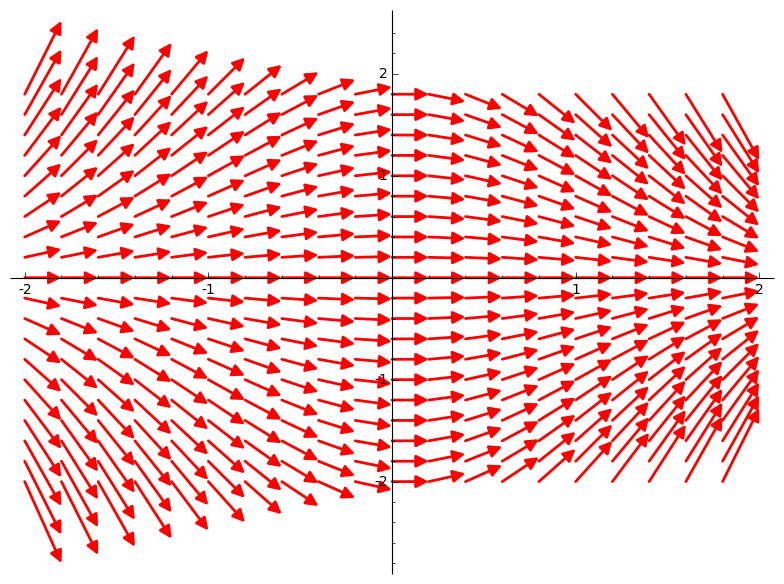
\includegraphics[scale=0.5]{figures/equadiff-courbe1.png}}
\only<2>{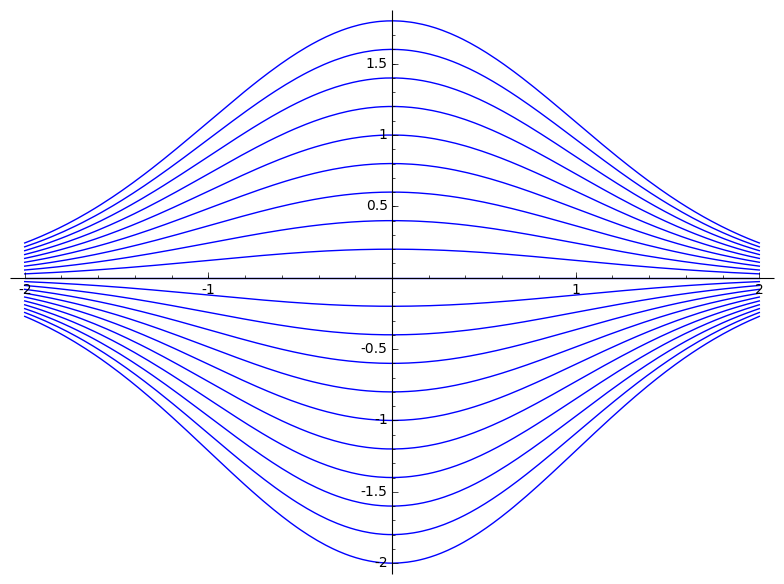
\includegraphics[scale=0.5]{figures/equadiff-courbe2.png}}
\only<3>{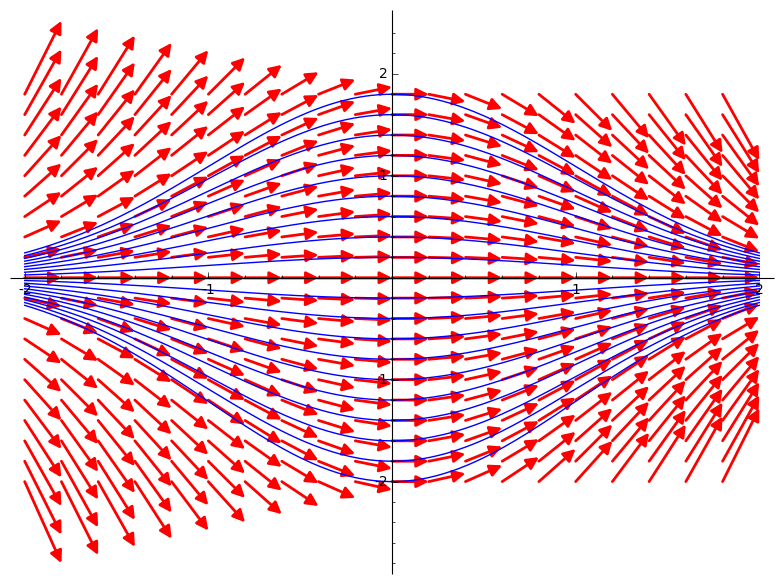
\includegraphics[scale=0.5]{figures/equadiff-courbe3.png}}
\only<4>{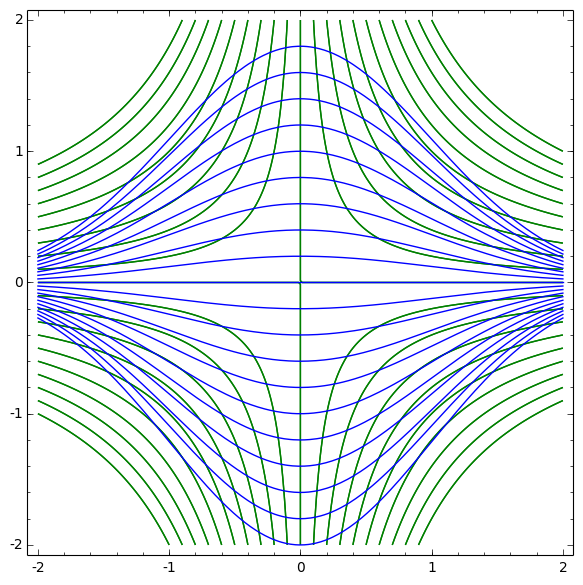
\includegraphics[scale=0.5]{figures/equadiff-courbe4.png}}
\end{center}

\end{frame}


\begin{frame}[fragile]

\begin{enumerate}
  \item Champ de vecteurs associé à $y' = f(x,y)$ :
   
\end{enumerate}
 
 % \insertcode{formel/Algos/equadiff-courbe-tex1.sage}{equadiff-courbe.sage (1)}
\begin{algo}[equadiff-courbe.sage (1)]
\begin{lstlisting}
def champ_vecteurs(f,xmin,xmax,ymin,ymax,delta):
    G = Graphics()  
    for i in srange(xmin, xmax, delta):
        for j in srange(ymin, ymax, delta):
            pt = vector([i,j])
            v = vector([1,f(u=i,v=j)])                 
            G = G + arrow(pt,pt+v)
    return G
\end{lstlisting}
\end{algo}  
\pause
  \begin{itemize}
    \item Les variables de la fonction $f$ sont ici $u$ et $v$
%\pause  
%    \item N'hésitez pas à renormaliser les vecteurs $v$ 
%\pause  
%    \item La fonction \codeinline{plot\_vector\_field}, prédéfinie dans \Sage, trace aussi les champs de
%  vecteurs
  \end{itemize}

\end{frame}



\begin{frame}

\begin{center}
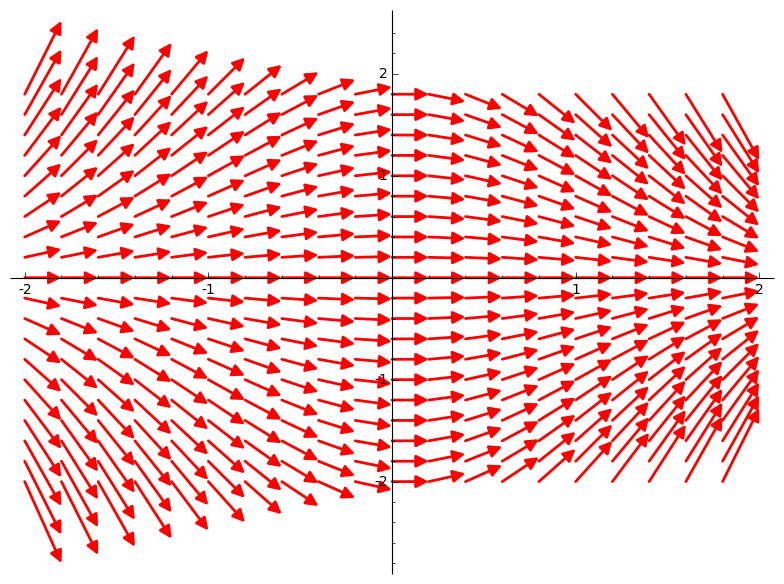
\includegraphics[scale=0.5]{figures/equadiff-courbe1.png}
\end{center}

\end{frame}



\begin{frame}[fragile] 
 
\begin{enumerate}
  \setcounter{enumi}{1}
  \item $y' = -xy$
  
  \pause
  \begin{enumerate}
    \item Les solutions de l'équation sont les
    $$y(x) = C \exp\left(-\frac{x^2}{2}\right) \quad \text{ où } \quad C \in \Rr$$
    
    
    \pause
    \item Le code suivant résout l'équation différentielle et trace la solution 
    avec la condition initiale $y(0)=k$, pour différentes valeurs de $k$
  \end{enumerate}
\end{enumerate} 
    
%\insertcode{formel/Algos/equadiff-courbe-tex2.sage}{equadiff-courbe.sage (2)}
\begin{algo}[equadiff-courbe.sage (2)]
\begin{lstlisting}
def courbes_integrales(equadiff,a,b,kmin,kmax,delta):
    G = Graphics()
    for k in srange(kmin, kmax, delta):
        sol = desolve(equadiff, y, ics=[0,k])
        G = G + plot(sol, (x, a, b))
    return G
\end{lstlisting}
\end{algo}      

 
\end{frame}


\begin{frame}

\evidence{Théorème d'existence et d'unicité de Cauchy-Lipschitz} 

Les courbes intégrales forment une partition 
de l'espace : par un point il passe exactement une courbe intégrale.

\begin{center}
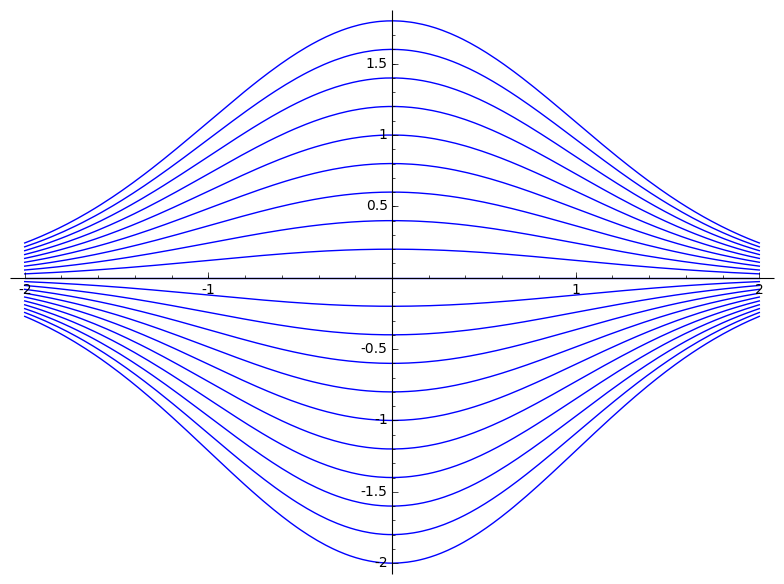
\includegraphics[scale=0.45]{figures/equadiff-courbe2.png}
\end{center}

\end{frame}



\begin{frame}  

\begin{enumerate}
\setcounter{enumi}{2}
  \item $y' = -xy$
  \begin{itemize}
    \item les isoclines sont définies par l'équation $f(x,y) = c$
    \pause
    \item elles se tracent par la commande \\
  \centerline{\codeinline{implicit\_plot(f-c, (x,xmin,xmax), (y,ymin, ymax))}}
  \pause
    \item ici les isoclines sont des hyperboles  d'équation $-xy=c$
  \end{itemize}
\end{enumerate}
\begin{center}  
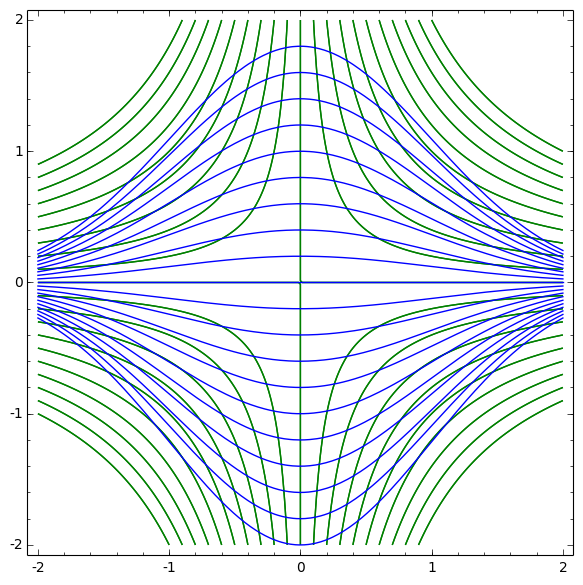
\includegraphics[scale=0.4]{figures/equadiff-courbe4.png}
\end{center}
\end{frame}



%%%%%%%%%%%%%%%%%%%%%%%%%%%%%%%%%%%%%%%%%%%%%%%%%%%%%%%%%%%%%%%%
\section{\'Equations différentielles du second ordre}

\begin{frame}
\begin{tp}
L'équation différentielle

\vspace*{-2ex}
$$x''(t) +f x'(t)+ \frac{k}{m} x(t) = 0$$ 
correspond au mouvement d'une masse $m$ 
attachée à un ressort de constante $k>0$
et subissant des frottements $f\ge0$.

Résoudre et tracer les solutions pour 
différentes valeurs de $f\ge0$ (prendre $k=1$, $m=1$) 
avec les conditions initiales :

\vspace*{-2ex}
$$x(0)= 1 \quad \text{ et } \quad x'(0)=0.$$
\end{tp}  

\myfigure{0.6}{
    \tikzinput{fig_formel_equadiff_ressort}   
}
\end{frame}


\begin{frame}


\begin{center}
\only<1>{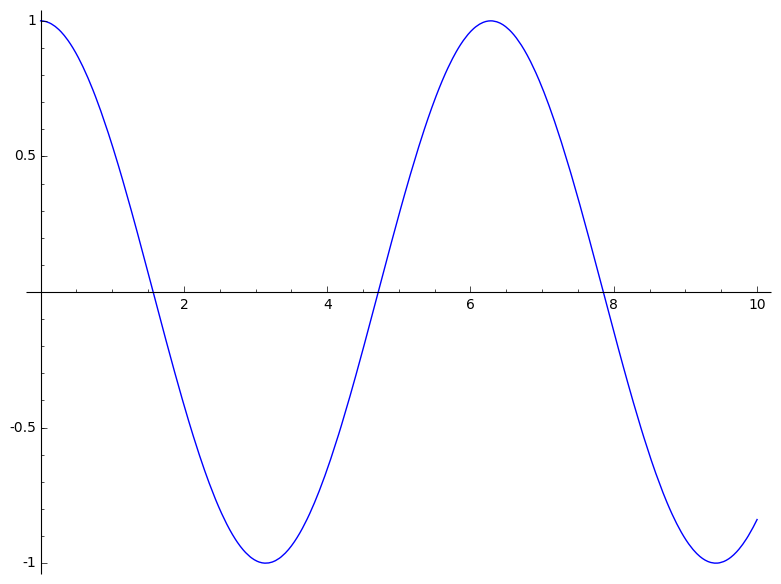
\includegraphics[scale=0.5]{figures/equadiff-ressort1.png}\\$f=0$}
\only<2>{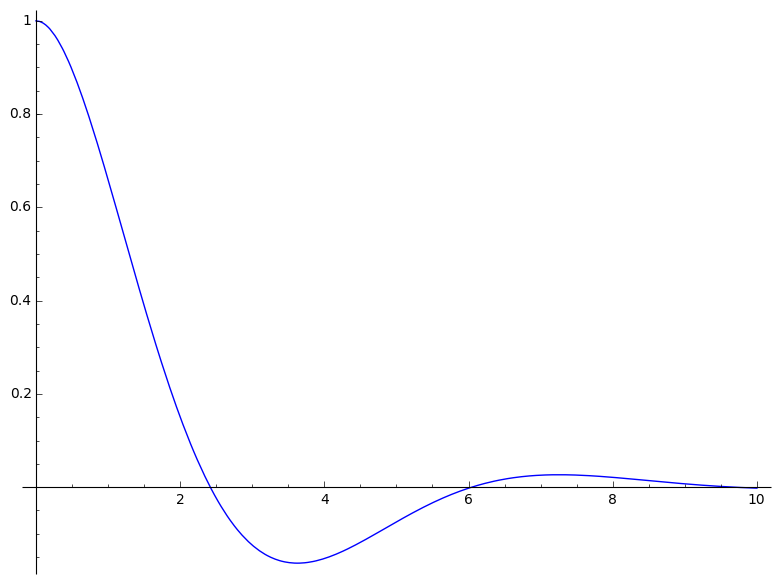
\includegraphics[scale=0.5]{figures/equadiff-ressort2.png}\\$f=1$}
\only<3>{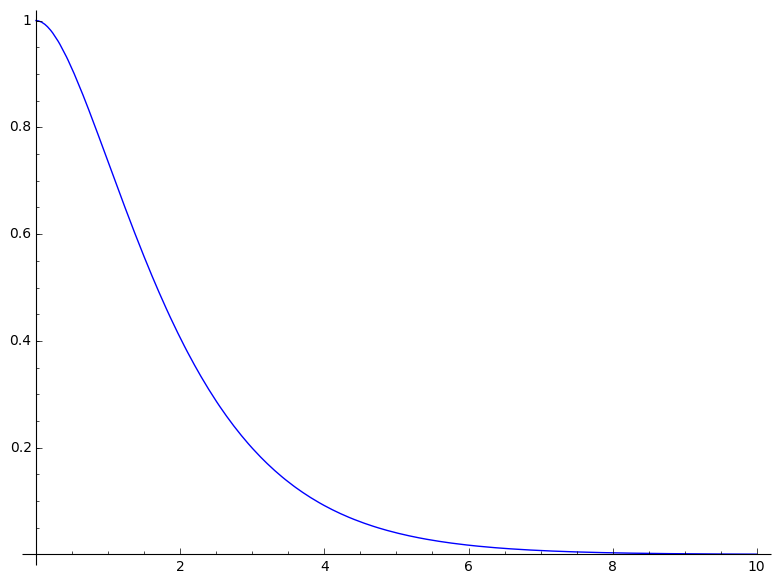
\includegraphics[scale=0.5]{figures/equadiff-ressort3.png}\\$f=2$} 
\end{center}

\end{frame}


\begin{frame}

Pour $f$ fixé, l'équation $x''(t) +f x'(t)+ \frac{k}{m} x(t) = 0$ se résout par : \\

{\small
\centerline{\codeinline{desolve(diff(x,t,2)+f*diff(x,t)+k/m*x(t) == 0, x, ics=[0,1,0])}}
}

\pause
\medskip

\begin{minipage}{0.7\textwidth}
\begin{itemize}
  \item Cas $f=0$. Pas de frottements
  \pause
  \begin{itemize}
    \item $x''+ \frac{k}{m} x = 0$
    \pause
    \item $k=1$, $m=1$ : $x''+ x = 0$
    \pause
    \item solutions $x(t) = \lambda \cos t + \mu \sin t$, $\lambda,\mu \in\Rr$
    \pause
    \item conditions initiales $x(0)=1$ et $x'(0)=0$
    \pause
    \item solution unique  $x(t) = \cos t$
  \end{itemize}  
\end{itemize}
\end{minipage}\pause
\begin{minipage}{0.29\textwidth}
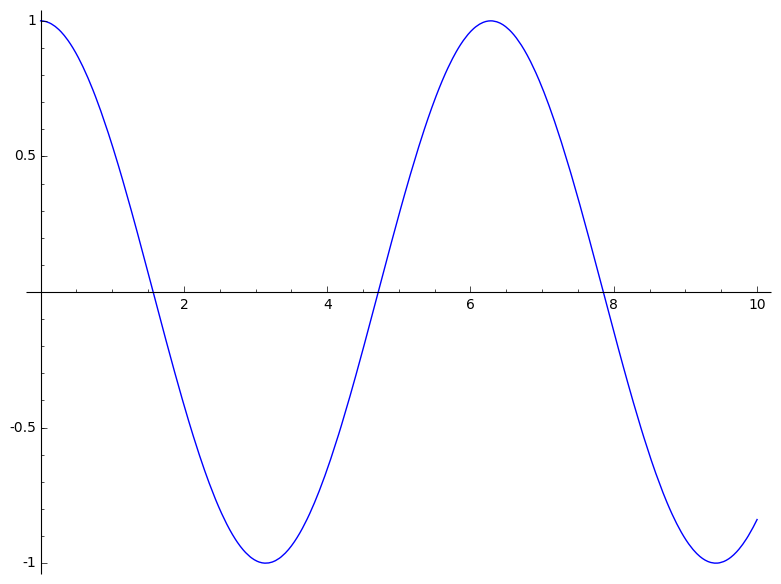
\includegraphics[scale=0.15]{figures/equadiff-ressort1.png}
\end{minipage}

\pause


\begin{minipage}{0.7\textwidth}
\begin{itemize}  
  \item Cas $0 < f < 2$. Frottements faibles
  
    \begin{itemize}
    \item $f=1$\pause
    \item $x(t)=\left(\frac{\sqrt{3}}{3} \sin\left(\frac{\sqrt{3}}{2} t\right) + 
   \cos\left(\frac{\sqrt{3}}{2} t\right)\right)
  e^{-\frac{1}{2} t}$
  \end{itemize}   
\end{itemize}
\end{minipage}\pause
\begin{minipage}{0.39\textwidth}
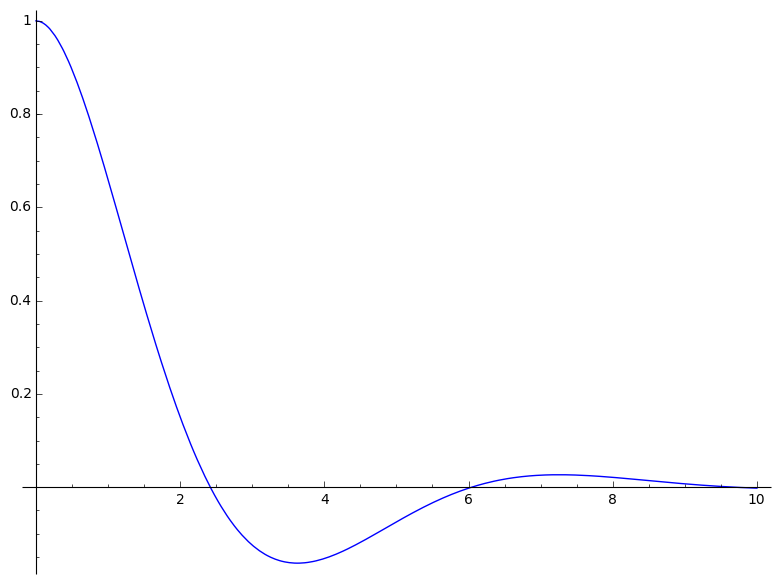
\includegraphics[scale=0.15]{figures/equadiff-ressort2.png}
\end{minipage}

\pause
\smallskip

\begin{minipage}{0.7\textwidth}
\begin{itemize}
  \item Cas $f \ge 2$. Frottements forts
  \begin{itemize}
  \pause
    \item $x(t) = (t + 1)e^{-t}$
  \end{itemize}     
\end{itemize}
\end{minipage}\pause
\begin{minipage}{0.29\textwidth}
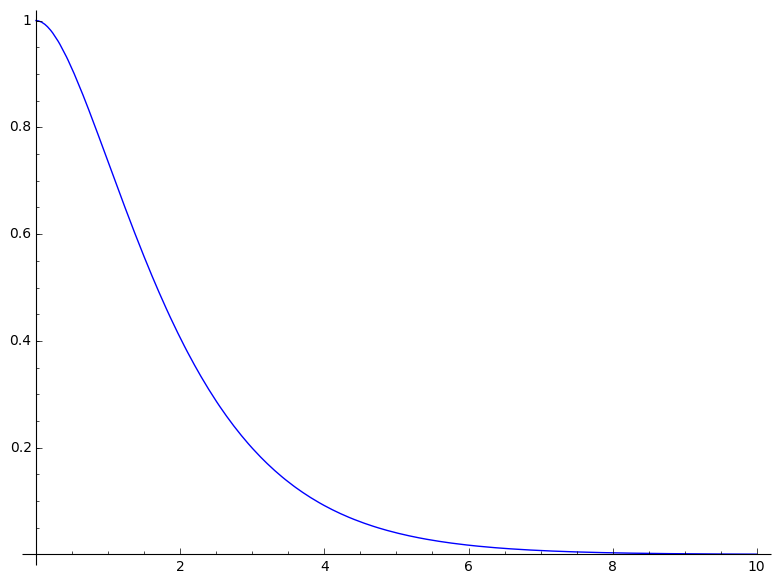
\includegraphics[scale=0.15]{figures/equadiff-ressort3.png}
\end{minipage}

\end{frame}




\end{document}
